\documentclass[a4paper,11pt]{article}
\usepackage{apacite}
\usepackage{url}
\usepackage{graphicx}
\graphicspath{ C:\Users\javie\Desktop\M6 }
\providecommand{\keywords}[1]{\textbf{\textit{Palabras clave---}} #1}
\begin{document}
\title{Espermatogénesis in vitro}
\author{Javier Villegas Salmerón- Universidad de Granada}
\maketitle
\section{Resumen}
$https://github.com/Javizuma/proyecto_final$\\
La generación de espermatozoides funcionales in vitro ha sido un objetivo durante casi un siglo. Hasta hace poco, los investigadores solo han logrado reproducir las primeras etapas de la espermatogénesis, lo que no es sorprendente dado que es un proceso que requiere esfuerzos combinados de las células germinales y varias células somáticas.
El proceso de espermatogénesis, si bien ha sido estudiado satisfactoriamente en diversas especies, ha sido especialmente investigado en ratones, pues este es el modelo animal  más interesante de cara a obtener conocimiento también sobre el ser humano debido a las similitudes que presentan ambas especies. Respecto al ciclo de espermatogénesis en si, existen diferencias, sobre todo en la duración del ciclo y obviamente derivadas de que los ratones son usados como modelos  precisamente porque tienen un tiempo de vida bastante corto que facilita su manejo y experimentación. 
En el siguiente articulo se realizará una reunión del conocimiento generado hasta el momento en esta rama y nos situaremos en el contexto de los estudios que se realizan actualmente. 
\keywords{Espermatogénesis, in vitro, PGCs}
\section{Introducción}
En ratón, los progenitores de las células primordiales germinales (PGCs) derivan del epiblasto (capa más gruesa del disco embrionario) del blastocisto (fase embrionaria) en el saco vitelino, en respuesta a la proteína BMP (proteína morfogénica ósea). Alrededor del día 6 embrionario, poco antes de que el epiblasto se separe en tres capas: ectodermo, mesodermo y endodermo, las células pluripotenciales de la zona posterior proximal del epiblasto se diferencian en PGCs. Tras esto, comienzan a migrar y entre los días 7 y 8 ya se encuentran en el alantoides (membrana que rodea el embrión), entonces son transferidas al epitelio del intestino grueso,  al día 9 o 10 empiezan a migrar al mesenterio (estructura que une intestino y abdomen), alcanzándolo al día 10 u 11. Por tanto, desde el intestino grueso alcanzan la cresta gonadal entre los días 9,5 y 11 y ya se les denomina como PGC postmigratorias. Sobre el día 13.5 se diferencian en proespermatogonias y estas quedan retenidas dentro del compartimento luminal de los túbulos seminíferos hasta el nacimiento. 
\subsection{Origen}

Tras el nacimiento las proespermatogonias comienzan su desarrollo y empieza la primera fase de la espermatogénesis. Sobre el primer o segundo día postnatal las proespermatogonias se diferencian en espermatogonias, así como migran hasta la periferia de los testículos y son flanqueadas por células somáticas de Sertoli dentro de los testículos y por las células mioides peritubulares que rodean la parte externa del cordón.

Las proteínas y las rutas de señalización involucradas en este proceso de migración aún se desconocen, pero se ha demostrado que la supresión de la señalización NOTCH (proteína transmembrana que permite la interacción entre distintos tipos celulares) en células de Sertoli es importante para mantener la quiescencia (es decir, que no migren de nuevo) en las proespermatogonias.
\subsection{Espermatogénesis}
El pool inicial de espermatogonias es heterogéneo, formado por células con distintos niveles de diferenciación durante los días 3 y 4 tras el nacimiento. Una pequeña fracción de estas formará las futuras células madre de la espermatogonia, asegurando una espermatogénesis continua durante toda la vida reproductiva del macho. Durante el proceso de espermatogénesis, la división de las células madre de la espermatogonia mantiene la población de células madre a la vez que produce una espermatogonia progenitora que sufrirá diferenciación.  Esta última aún posee una cierta conexión tubular, por lo que se forma un puente intercelular que resulta en una citocinesis incompleta. Estos puentes están muy conservados evolutivamente y permiten el intercambio de moléculas entre células dentro del coenocito.

La obligación de entrar en meiosis se produce con la transición de espermatogonias no diferenciadas a sí diferenciadas, a estas se les denomina A1. Por mitosis estas forman las A2, que a su vez se dividen y crean las A3 que se dividen y generan las A4.  Las próximas dos divisiones mitóticas forman las espermatogonias intermedias y las B. La espermatogonia B resultante entra en la primera profase de la meiosis como espermatocito preleptotene (siendo el leptotene la fase inicial de la profase I, constituida por leptotene, cigotene, paquitene diplotene y diacinesis). La fase meiótica es bastante larga, con un periodo de alrededor 13 días, donde aproximadamente la mitad de los túbulos seminíferos contendrán células que se encuentren en el estado paquiteno tardío (paquiteno es la tercera subfase de la profase). Las espermátidas (primeras células tras la meiosis) no se detectan hasta el día 20 o 21 post natal, y durante los siguientes 13 días estas se diferencian en espermátidas elongadas y el primer esperma con capacidad de fertilizar óvulos se puede observar sobre el día 35 post natal.
\section{Estado del Arte: Aplicaciones espermatogénesis in vitro}
La infertilidad se ha convertido en un problema de salud global, y esta se debe en un 40-50\% de las ocasiones a factores que afectan al hombre. Dentro de estos factores encontramos factores genéticos, del entorno o incluso a tratamientos tóxicos para las gónadas. No obstante, el desarrollo de la biotecnología reproductiva está abriendo nuevas vías para rescatar la fertilidad y posibilitar la paternidad en muchos casos. La producción in vitro de células germinales haploides masculinas ha demostrado ser una herramienta muy útil no solo para los casos de oligozoospermia (pocos espermatozoides) o azoospermia (ausencia total de espermatozoides), sino también para la conservación de fertilidad en niños que aún no han alcanzado la pubertad y que tienen que afrontar un tratamiento que produce efectos tóxicos sobre las gónadas. 
\subsection{Pacientes de cáncer prepubertad}
Los tratamientos frente al cáncer llevan asociados un riesgo considerable para la fertilidad, por lo que el control de la toxicidad de estos tratamientos se ha vuelto un punto interesante de estudio( en un primer momento lo que se hacía era la preservación del semen pero esta opción no existe para los pacientes que aún no han alcanzado la pubertad). Para ellos existen dos vías:
-Minimizar el daño testicular o proteger las SSC in vivo
Se han tratado de utilizar medicamentos citoprotectores pero hasta la fecha no hay ninguno disponible para humanos.
-Criopreservar tejido testicular
Por tanto la única alternativa es la criopreservación de tejido testicular. Este tejido contiene las SSC, que se pueden obtener por digestión enzimática del tejido testicular (viabilidad del 60%).
No obstante, hay un problema inherente a esta técnica que deriva del hecho que las SSC tienen el riesgo de convertirse en células madres pluripotentes que generen teratomas. Una posible solución a esto sería conseguir una espermatogénesis completa y segura in vitro que nos permita usar SSCs criopreservadas para luego utilizar con técnicas como ISCI o ROSI.  
Además, presenta ventajas respecto a la criopreservación de esperma: las SSC están menos diferenciadas que los espermatozoides, siendo fáciles de expandir in vitro y permitiendo ser transferidas de vuelta al paciente, y además, se conserva todo el genoma del individuo, lo que no sucede en los espermatozoides. 
\begin{figure}[htb!] 
    \caption{PACIENTES DE CÁNCER PREPUBERTAD}
    \centering 
    \includegraphics[width=5cm]{cancer-prepuber.jpg}
\end{figure}
\subsection{Generación de esperma funcional a partir de una célula madre pluripotente inducida}
\begin{figure}[htb!] 
    \caption{Generación de esperma funcional a partir de una célula madre pluripotente inducida}
    \centering 
    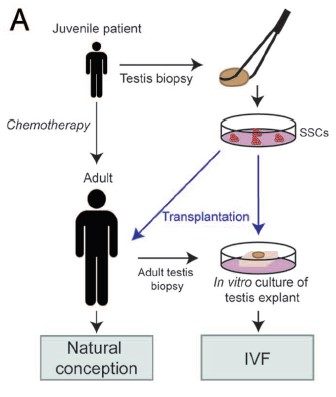
\includegraphics[width=5cm]{Cancer-prepuber.jpg}
\end{figure}
El descubrimiento de métodos para generar células similares a células totipotenciales, células ES, a partir de células madre pluripotente inducidas , células iPS, ha abierto las puertas a otro medio para generar espermátidas funcionales in vitro. La belleza de esta técnica radica en que no es necesario obtener tejido testicular del paciente. En la forma en que se contempla este enfoque, las células iPS serían inducidas por el linaje celular de las células germinales masculinas utilizando métodos in vitro que ya han sido desarrollados. 
A continuación de la purificación de las células germinales que se habían diferenciado parcialmente in vitro a partir de las células iPS, serían empujadas aún más hacia la madurez a través de su trasplante en explantes de testículo de otro individuo. Esto es necesario porque las técnicas actuales in vitro no son lo suficientemente eficientes. Para terminar las células que progresen más allá de la fase haploide serán aisladas y usadas para fertilizar óvulos a través de ICSI o ROSI.

\subsection{Terapia génica para obtener esperma fértil de hombres infértiles}
Otra forma de obtención de esperma fértil de un hombre infértil sería la utilización de las técnicas in vitro junto a terapia génica. En el caso de un hombre infértil, si conocemos la mutación causante, esta podría ser modificada en sus células germinales in vitro, para posteriormente volver a ser introducidas en el paciente o cultivadas in vitro, de formas que se conviertan en fértiles y funcionales. 
Este tipo de técnicas podría tener resultados impredecibles ya que al modificar un gen en concreto no podemos saber con certeza el resultado que tendrá en el resto, y a la vez estaríamos hablando de modificar el genoma humano, lo que levanta varios dilemas éticos. 
\begin{figure}[htb!] 
    \caption{Terapia génica para obtener esperma fértil de hombres infértiles}
    \centering 
    \includegraphics[width=5cm]{cancer-prepuber.jpg}
\end{figure}
\end{document}